\documentclass{almostllncs}

%%%%%%%%%% PACKAGES
\usepackage{comment}
\usepackage{booktabs}                           
%\usepackage{subcaption} 
\usepackage{mathtools}
\usepackage{amsmath}
\usepackage{amssymb}
\usepackage{amsfonts}
\usepackage{prftree}
\usepackage{newtxtext}
\usepackage{newtxmath}
\usepackage[bbgreekl]{mathbbol} % must go after newtxtext & newtxmath
\usepackage{tikz}\usetikzlibrary{arrows}\usepgflibrary{arrows}
\usepackage{tabularx,multirow}
\usepackage{xspace}
\usepackage{wrapfig}
\usepackage{array}
\usepackage{todonotes}
\usepackage[normalem]{ulem}
\usepackage{multicol}
\usepackage{thmtools} 
\usepackage{thm-restate}
\usepackage{stmaryrd}
\usepackage{url}
\usepackage[hidelinks]{hyperref}
\usepackage{listings}% http://ctan.org/pkg/listings
\lstset{
	basicstyle=\ttfamily,
	mathescape
}
\usepackage{algorithm2e}
\usepackage{enumitem}
\usepackage[nocompress]{cite}

% for dealing with underscores
\usepackage[T1]{fontenc}

%%%%%%%%%% UNCLASSIFIED
% text
\newcommand{\BMC}{Bounded Model Checking\xspace}
\newcommand{\MmuL}{Matching $\mu$-Logic\xspace}
\newcommand{\mmul}{matching $\mu$-logic\xspace}
\newcommand{\ml}{matching logic\xspace}
\newcommand{\ModmuL}{Modal $\mu$-Logic\xspace}
\newcommand{\modmul}{modal $\mu$-logic\xspace}
\newcommand{\PS}{\mathcal{H}}
\newcommand{\nats}{\mathbb{N}} % set of natural numbers
\makeatletter % Roman numerals
\newcommand{\rmnum}[1]{\romannumeral #1}
\newcommand{\Rmnum}[1]{\expandafter\@slowromancap\romannumeral #1@}
\newcommand*{\rom}[1]{\expandafter\@slowromancap\romannumeral #1@}
\makeatother
\newcommand{\K}{$\mathbb{K}$\xspace} % \K framework
\newcommand{\doubleslash}{//\xspace}
\newcommand{\LTL}{\textsf{LTL}\xspace}
\newcommand{\CTL}{\textsf{CTL}\xspace}

% basic math
\newcommand{\pset}[1]{\mathcal{P}(#1)} % powerset
\newcommand{\cln}{\mathord{:}}
\newcommand{\ldot}{\mathord{.}}
\newcommand{\imp}{\to}
\newcommand{\dimp}{\leftrightarrow}
\newcommand{\setsymdiff}{\mathbin{\triangle}}
\newcommand{\FV}{\mathit{FV}}
\newcommand{\To}{\Rightarrow}

% an implementation of widebar
% obtained from [[https://tex.stackexchange.com/questions/16337/
% can-i-get-a-widebar-without-using-the-mathabx-package]]
\makeatletter
\let\save@mathaccent\mathaccent
\newcommand*\if@single[3]{%
	\setbox0\hbox{${\mathaccent"0362{#1}}^H$}%
	\setbox2\hbox{${\mathaccent"0362{\kern0pt#1}}^H$}%
	\ifdim\ht0=\ht2 #3\else #2\fi
}
%The bar will be moved to the right by a half of \macc@kerna, which is computed 
%by amsmath:
\newcommand*\rel@kern[1]{\kern#1\dimexpr\macc@kerna}
%If there's a superscript following the bar, then no negative kern may follow 
%the bar;
%an additional {} makes sure that the superscript is high enough in this case:
\newcommand*\widebar[1]{\@ifnextchar^{{\wide@bar{#1}{0}}}{\wide@bar{#1}{1}}}
%Use a separate algorithm for single symbols:
\newcommand*\wide@bar[2]{\if@single{#1}{\wide@bar@{#1}{#2}{1}}{\wide@bar@{#1}{#2}{2}}}
\newcommand*\wide@bar@[3]{%
	\begingroup
	\def\mathaccent##1##2{%
		%Enable nesting of accents:
		\let\mathaccent\save@mathaccent
		%If there's more than a single symbol, use the first character instead 
		%(see below):
		\if#32 \let\macc@nucleus\first@char \fi
		%Determine the italic correction:
		\setbox\z@\hbox{$\macc@style{\macc@nucleus}_{}$}%
		\setbox\tw@\hbox{$\macc@style{\macc@nucleus}{}_{}$}%
		\dimen@\wd\tw@
		\advance\dimen@-\wd\z@
		%Now \dimen@ is the italic correction of the symbol.
		\divide\dimen@ 3
		\@tempdima\wd\tw@
		\advance\@tempdima-\scriptspace
		%Now \@tempdima is the width of the symbol.
		\divide\@tempdima 10
		\advance\dimen@-\@tempdima
		%Now \dimen@ = (italic correction / 3) - (Breite / 10)
		\ifdim\dimen@>\z@ \dimen@0pt\fi
		%The bar will be shortened in the case \dimen@<0 !
		\rel@kern{0.6}\kern-\dimen@
		\if#31
		\overline{\rel@kern{-0.6}\kern\dimen@\macc@nucleus\rel@kern{0.4}\kern\dimen@}%
		\advance\dimen@0.4\dimexpr\macc@kerna
		%Place the combined final kern (-\dimen@) if it is >0 or if a 
		%superscript follows:
		\let\final@kern#2%
		\ifdim\dimen@<\z@ \let\final@kern1\fi
		\if\final@kern1 \kern-\dimen@\fi
		\else
		\overline{\rel@kern{-0.6}\kern\dimen@#1}%
		\fi
	}%
	\macc@depth\@ne
	\let\math@bgroup\@empty \let\math@egroup\macc@set@skewchar
	\mathsurround\z@ \frozen@everymath{\mathgroup\macc@group\relax}%
	\macc@set@skewchar\relax
	\let\mathaccentV\macc@nested@a
	%The following initialises \macc@kerna and calls \mathaccent:
	\if#31
	\macc@nested@a\relax111{#1}%
	\else
	%If the argument consists of more than one symbol, and if the first token is
	%a letter, use that letter for the computations:
	\def\gobble@till@marker##1\endmarker{}%
	\futurelet\first@char\gobble@till@marker#1\endmarker
	\ifcat\noexpand\first@char A\else
	\def\first@char{}%
	\fi
	\macc@nested@a\relax111{\first@char}%
	\fi
	\endgroup
}
\makeatother

% mathsc fonts
\newcommand{\mathsc}[1]{{\normalfont\textsc{#1}}} % small caps in math mode
\newcommand{\Var}{\mathsc{Var}}
\newcommand{\EVar}{\mathsc{EVar}}
\newcommand{\SVar}{\mathsc{SVar}}
\newcommand{\PVar}{\mathsc{PVar}}
\newcommand{\Pattern}{\mathsc{Pattern}}

% mathsf/textsf fonts
\newcommand{\TS}{\textnormal{\textsf{TS}\xspace}}
\newcommand{\RS}{\textnormal{\textsf{RS}\xspace}}
\newcommand{\Lang}{\textnormal{\textsf{Lang}\xspace}}
\newcommand{\cfg}{\textnormal{\textsf{cfg}\xspace}}
\newcommand{\init}{\textnormal{\textsf{init}\xspace}}
\newcommand{\prop}{\textnormal{\textsf{prop}\xspace}}
\newcommand{\pattern}{\textnormal{\textsf{pattern}\xspace}}
\newcommand{\predicate}{\textnormal{\textsf{predicate}\xspace}}
\newcommand{\sub}{\textnormal{\textsf{sub}\xspace}}
\newcommand{\IMP}{{\mathsf{IMP}}}

% mathcal font
\newcommand{\Acal}{\mathcal{A}}
\newcommand{\Ccal}{\mathcal{C}}
\newcommand{\Fcal}{\mathcal{F}}
\newcommand{\Qcal}{\mathcal{Q}}

% mathbb font
\newcommand{\Sbb}{\mathbb{S}}

% sorts using mathit fonts
\newcommand{\Cfg}{\mathit{Cfg}}
\newcommand{\State}{\textit{State}}

% symbol
\newcommand{\rhobar}{\bar{\rho}}
\newcommand{\sig}{\mathbb{\Sigma}}
\newcommand{\sigmaM}{\sigma_M}
\DeclarePairedDelimiter{\ceil}{\lceil}{\rceil}
\DeclarePairedDelimiter{\floor}{\lfloor}{\rfloor}
\DeclarePairedDelimiter{\bracket}{\llbracket}{\rrbracket}

% contexts
\newcommand{\CSub}[1]{C_{#1}}
\newcommand{\Csigma}{\CSub{\sigma}}
\newcommand{\Csigmaapp}[1]{\CSub{\sigma}[#1]}

% name of the proof rules
\newcommand{\prule}[1]{\textnormal{\textsc{(#1)}}}

\newcommand{\modusponens}{\prule{Modus Ponens}\xspace}
\newcommand{\propagationbottom}{\prule{Propagation$_\bot$}\xspace}
\newcommand{\propagationvee}{\prule{Propagation$_\vee$}\xspace}
\newcommand{\framing}{\prule{Framing}\xspace}
\newcommand{\existence}{\prule{Existence}\xspace}
\newcommand{\singletonvariable}{\prule{Singleton Variable}\xspace}
\newcommand{\step}{\prule{STEP}\xspace}

% modalities
\newcommand{\wnext}{{\circ}}
\newcommand{\snext}{{\bullet}}
\newcommand{\eventually}{{\lozenge}}
\newcommand{\always}{{\square}}
\newcommand{\until}{\mathbin{U}}
\newcommand{\wellfounded}{{\mathsf{WF}}}


\begin{document}

\title{\large{Proof-carrying \BMC{} for All languages}}

\subtitle{\normalsize{Thesis Proposal}}

\author{Yi Zhang}
\institute{University of Illinois at Urbana-Champaign}

\maketitle

\begin{abstract}
Model checking has been used extensively to algorithmically check temporal property of models.
Research on software (bounded) model checking has been focusing on various techniques(e.g., symbolic model checking, predicate abstraction, partial order reduction, etc.) to solve the state-space explosion problem.
Various tools such as SLAM, CBMC and CORRAL were proposed.
There are two major problems shared among these tools: 1) They only support specific programming languages 2) There is no guarantee that the implementations of the model checkers are correct.
To solve the problems, my thesis proposes a proof-carrying bounded model checker for all languages.
We can encode both the operational semantics of a language and \modmul as theories and notations in \mmul.
As a result, bounded model checking becomes a strategy for searching the proof for a given pattern within \emph{k} step.
The model checker for a language can be obtained for free once the operational semantics for that language is defined.
The result of bounded model checking a pattern is an proof object which is checkable by an external proof checker.
Moreover, since the bounded model checker is derived from the actual operational semantics, there is no discrepancy between the model checker and the actual language semantics.
This proposal document describes the work that I have done so far towards this goal, and my proposed plan for the rest of the thesis work.

\end{abstract}

\section{Introduction}
Model checking has been used extensively to algorithmically check temporal property of models.
Early application of model checking were in hardware and protocol design.
Later the idea was applied to software.
Due to the advent of sophisticated SAT and SMT solvers, symbolic model checking becomes a popular approach to cope with infinite program states.
Various techniques and tools were proposed and many tools such as SLAM~\cite{SLAM} and CORRAL~\cite{corral-a-solver-for-reachability-modulo-theories-2} are used in the daily development in companies like Microsoft.
Most of the model checking tools were developed for a fixed target language, and the language semantics is usually hardcoded within the implementation of their model checking algorithms.
Due to their monolithic design nature, retargeting them to another language requires significant effort.
There are two approaches to retarget the model checker to a new language.
One is to replace the hardcoded language semantics with the new target language semantics, which may requires substantial amount of work.
The other approach is to implement a translator from the new language to the existing language, which has its own limitation if the new language is quite different from the existing one.
Moreover, since the language semantics is hardcoded in the model checker, it is very hard to test the hardcoded semantics conforming to the actual behavior of the code, let alone there is no guarantee on the correctness of the tool itself.

The recent work~\cite{chen-rosu-2019-lics} on \mmul shows various logic including \modmul can be defined as theories in \mmul.
This suggests that \mmul offers a unifying playground to specify properties and reason about transition systems.
Since operational semantics already provides the transition relation between program states, it is natural to build a (bounded) model checker for all languages based on operational semantics in \mmul.
This approach admits several advantages.
First, the model checker is language-independent and highly reusable.
In addition, operational semantics is executable and thus it can be easily tested.
Since the model checker is automatically derived from the operational semantics, there is no need to worry about the discrepancies between the model checker and the actual behavior of the code.
Second, we formalized the bounded model checking as a strategy to search proof for a given pattern in the \mmul proof system within \emph{k} step.
Each step in the model checking algorithm can be justified by a \mmul proof rule.
In the end, the model checker is able to produce a proof object which is checkable by an external proof checker.
As a result, there is no need to trust the implementation of the model checker anymore.

The goal of my thesis is to demonstrate and improve the scalability and
practicality of such language-independent bounded model checker.
Specific work to support this goal falls into these categories:

\begin{itemize}
\item Implementing the language-independent model checker and proof generation.
\item Instantiating the model checker by plugging-in various real-world programming language semantics and improving its performance.
\item Applying the derived model checker to real-world systems and applications, demonstrating their practical feasibility both in isolation and by comparison to state-of-the-art tools specifically crafted for the target languages.
\end{itemize}

\section{Background}
This section presents the preliminaries of \mmul and \modmul.

\subsection{\MmuL Preliminaries}
The recent work \cite{chen-rosu-2019-lics} proposed \mmul, an extension of \ml \cite{matching-logic-17} with a least fixpoint $\mu$-binder.
It is shown that \mmul captures many important logics as special instances, including \modmul as well as dynamic logic and various temporal logic.
Therefore, \mmul serves as a unifying foundation for specifying and reasoning about fixpoints and induction, programming languages and various program analysis.

\subsubsection{\MmuL syntax}

\begin{definition} \label{def:MmuL-syntax}

A \emph{matching $\mu$-logic signature} or simply a \emph{signature}
$\sig = (S, \Var, \Sigma)$ is a triple.
$S$ is a nonempty set of \emph{sorts}.
$\Var = \{ \EVar_s \}_{s \in S} \cup \{ \SVar_s \}_{s \in S}$ is a disjoint union of two $S$-indexed sets of variables:
the \emph{element variables} denoted as $x \cln s$, $y \cln s$, etc.
in $\EVar$, and
the \emph{set variables} denoted as $X \cln s, Y \cln s$, etc
in $\SVar$.
$\Sigma = \{ \Sigma_{s_1 \dots s_n , s} \}_{s_1,\dots,s_n,s \in S}$ is an $(S^* \times S)$-indexed set of countably many \emph{many-sorted symbols}.
When $n = 0$, we write $\sigma \in \Sigma_{\lambda,s}$ and say $\sigma$ is a \emph{constant}.
Matching $\mu$-logic \emph{$\sig$-patterns}
or simply \emph{($\sig$-)patterns}
are defined inductively for all sorts
$s, s',s_1,\dots,s_n\in S$ as follows:
\begin{align*}
\varphi_s 
& \Coloneqq 
x \cln s \in \EVar_s \mid
X \cln s \in \SVar_s \mid
\varphi_s \wedge \varphi_s \mid
\neg \varphi_s \mid
\exists x \cln s' \ldot \varphi_s \\
& \ \  \mid
\sigma(\varphi_{s_1},\dots,\varphi_{s_n})
\quad \text{if $\sigma \in \Sigma_{s_1\dots s_n , s}$} \\
& \ \  \mid
\mu X \cln s \ldot \varphi_s
\quad \text{if $\varphi_s$ is positive in $X \cln s$},
\end{align*}
\noindent
Note that we only quantify over element variables, not set variables.
We say $\varphi_s$ is \emph{positive} in $X \cln s$ if
every free occurrence of $X \cln s$ is under an even number of negations.
We let $\Pattern(\sig) = \{ \Pattern_s \}_{s \in S}$ denote the set of
all matching $\mu$-logic $\sig$-patterns and feel free
to drop the signature $\sig$.

\end{definition}

We first give some intuition about the patterns in \mmul and then formalize its semantics in Definition~\ref{def:MmuL-semantics}.
Intuitively, patterns evaluate to the sets of elements that \emph{match} them.
An element variable $x \cln s$ is a pattern that is matched by exactly one element;
A set variables $X \cln s$ evaluates to \emph{set}.
$\varphi_1 \wedge \varphi_2$ is matched by elements
matching both $\varphi_1$ and $\varphi_2$;
$\neg \varphi$ is matched by elements not matching $\varphi$;
$\exists x \cln s' \ldot \varphi$ is a pattern that allows us to
abstract away irrelevant parts (i.e., $x \cln s'$) of the
structures, which can match patterns 
$\sigma(\varphi_{s_1},\dots,\varphi_{s_n})$.
The least fixpoint pattern $\mu X \cln s \ldot\, \varphi_s$ gives
\emph{the least solution} (under set containment) of the equation 
$X \cln s = \varphi_s$ of set variable $X \cln s$
(this should be taken as merely intuition at this stage, because we may not 
have equality in the theories).
The condition of positive occurrence guarantees the existence of such a least solution.

We adopt the following derived constructs as syntactic sugar:
\begin{align*}
&\varphi_1 \vee \varphi_2 \equiv \neg (\neg \varphi_1 \wedge \neg \varphi_2)
&& \forall x \cln s \ldot \varphi \equiv 
\neg \exists x \cln s \ldot \neg \varphi
\\
& \varphi_1 \imp \varphi_2 \equiv \neg \varphi_1 \vee \varphi_2
&& \top_s \equiv \exists x \cln s \ldot x \cln s
\\
& \varphi_1 \dimp \varphi_2 \equiv (\varphi_1 \imp \varphi_2)
\wedge (\varphi_2 \imp \varphi_1)
&& \bot_s \equiv \neg \top_s
\\
& \nu X \cln s \ldot \varphi_s \equiv \neg \mu X \cln s \ldot \neg 
\varphi_s[\neg X \cln s / X \cln s]
\end{align*}
\noindent
Intuitively, $\varphi_1 \! \vee \! \varphi_2$ is matched by elements matching $\varphi_1$ or $\varphi_2$;
$\top_s$ is matched by all elements (in the sort universe $s$);
and $\bot_s$ is matched by no elements.
We drop sort $s$ whenever possible, so we write $x, \top, \bot$ instead of $x \cln s, \top_s, \bot_s$.

\subsubsection{\MmuL semantics}
In \mmul, symbols are interpreted as {\em relations}, and thus \mmul patterns
evaluate to {\em sets of elements} (those ``matching'' them).

\begin{definition} \label{def:Mmul-models}

Given $\sig = (S,\Sigma)$, a \emph{\mmul $\sig$-model} 
$M = (\{ M_s \}_{s \in S}, \{\sigma_M\}_{\sigma\in\Sigma})$,
or simply a \emph{($\sig$)-model}, contains
\begin{itemize}	
\item a nonempty carrier set $M_s$ for each sort $s \in S$;
\item an interpretation $\sigma_M \colon M_{s_1} \times \dots \times M_{s_n} \to \pset{M_s}$
	  for each $\sigma \in \Sigma_{s_1 \dots s_n , s}$, where $\pset{M_s}$ is the powerset of $M_s$.
\end{itemize}

\end{definition}

\noindent
We overload the letter $M$ to also mean the $S$-indexed set $\{ M_s \}_{s \in S}$.
We tacitly
use the same letter $\sigma_M$ to mean its \emph{pointwise extension},
$\sigma_M \colon \pset{M_{s_1}} \times \dots \times \pset{M_{s_n}} \to
\pset{M_s}$, defined as:
$$
\sigma_M(A_1,\dots,A_n) = {\bigcup} \{ \sigma_M (a_1,\dots,a_n) \mid
a_1 \in A_1,\dots, a_n \in A_n \}
$$
for all $A_1 \subseteq M_{s_1}, \dots, A_n \subseteq M_{s_n}$.

\begin{proposition}\label{prop:property_of_propagation_semantics}

For all $A_i,A'_i \subseteq M_{s_i}$, $1 \le i \le n$, the pointwise extension $\sigma_M$ has the following \emph{property of propagation}:
\vspace*{-0.3em}
\begin{align*}
&\sigma_M(A_1,\dots,A_n) = \emptyset 
\text{ if $A_i = \emptyset$ for some $1 \le i \le n$},
\\
&\sigma_M(A_1 \cup A'_1 ,\dots, A_n \cup A'_n)
= \textstyle{\bigcup_{1 \le i \le n, B_i \in \{ A_i, A'_i \}}} \sigma_M(B_1,\dots,B_n),
\\
&\sigma(A_1,\dots,A_n) \subseteq \sigma(A'_1,\dots,A'_n)
\text{ if $A_i \subseteq A'_i$ for all $1 \le i \le n$}.
\end{align*}

\end{proposition}

\begin{definition}\label{def:MmuL-semantics}

Let $\sig = (S, \Var, \Sigma)$ be a signature with $\Var = \EVar \cup \SVar$,
and $M = ( \{ M_s \}_{s \in S} , \{\sigma_M\}_{\sigma\in\Sigma} )$ be a $\sig$-model.
A \emph{valuation} $\rho \colon \Var \to (M \cup \pset{M})$ is a function such that $\rho(x) \in M_s$ for all $x \in \EVar_s$ and $\rho(X) \in \pset{M_s}$ for all $X \in \SVar_s$.
Its \emph{extension} $\rhobar \colon \Pattern \to \pset{M}$ can be inductively defined as:
\begin{itemize}
\item $\rhobar(x) = \{\rho(x)\}$ \space for all $x \in \EVar_s$;
\item $\rhobar(X) = \rho(X)$ \space for all $X \in \SVar_s$;
\item $\rhobar(\varphi_1 \wedge \varphi_2) = \rhobar(\varphi_1) \cap \rhobar(\varphi_2)$,
      \space for $\varphi_1,\varphi_2 \in \Pattern_s$;
\item $\rhobar(\neg \varphi) = M_s \setminus \rhobar(\varphi)$
      \space for all $\varphi \in \Pattern_s$;
\item $\rhobar(\exists x \ldot \varphi) = \bigcup_{a \in M_{s'}}       \widebar{\rho[a/x]}(\varphi)$ \space for all $x \in \Var_{s'}$;
\item $\rhobar(\sigma(\varphi_1 ,..., \varphi_n))
= \sigmaM( \rhobar(\varphi_1) ,..., \rhobar(\varphi_n) )$
\space for $\sigma \in \Sigma_{s_1 \dots s_n , s}$;
\item $\rhobar(\mu X \ldot \, \varphi) = \mu \Fcal^\rho_{\varphi,X}$
	  \space for all $X \in \SVar_s$, where 
	  $\Fcal^\rho_{\varphi,X}(A) = \widebar{\rho[A/X]}(\varphi)$ 
	  for all $A \subseteq M_s$.
\end{itemize}
\noindent
where ``$\setminus$'' is set difference, $\rho[a/x]$ denotes
the $M$-valuation $\rho'$ with 
$\rho'(x) = a$ and $\rho'(y) = \rho(y)$ for all $y \not\equiv x$
and $\rho[A/X]$ is the $\rho'$ with
$\rho'(X) = A$ and $\rho'(Y) = \rho(Y)$ for all $Y \not\equiv X$.
Note $\Fcal^\rho_{\varphi,X}$ is monotone, since $\varphi$ is positive in $X$.

\end{definition}

\begin{proposition}\label{prop:expected_semantics}

The following propositions hold:
\begin{itemize}
\item $\rhobar(\top_s) = M_s$ and $\rhobar(\bot_s) = \emptyset$;
\item $\rhobar(\varphi_1 \vee \varphi_2) = \rhobar(\varphi_1) \cup \rhobar(\varphi_2)$;
\item $\rhobar(\varphi_1 \! \imp \varphi_2) = M_s \setminus (\rhobar(\varphi_1) \setminus \rhobar(\varphi_2))$
	  \space for $\varphi_1,\varphi_2 \in \Pattern_s$;
\item $\rhobar(\varphi_1 \! \dimp \varphi_2) = M_s \setminus (\rhobar(\varphi_1) \setsymdiff \rhobar(\varphi_2))$
	  \space for $\varphi_1,\varphi_2 \in \Pattern_s$;
\item $\rhobar(\forall x \ldot \varphi) = \bigcap_{a \in M_{s'}} \widebar{\rho[a/x]}(\varphi)$,
	  \space for all $x \in \Var_{s'}$;
\end{itemize}
\noindent
where ``$\setsymdiff$'' is set symmetric difference.

\end{proposition}

\begin{definition} \label{def:MmuL-validity}
	
We say pattern $\varphi$ is \emph{valid} in $M$, written $M \vDash \varphi$,
iff $\rhobar(\varphi) = M$ for all $\rho \colon \Var \to M$.
Let $\Gamma$ be a set of patterns called \emph{axioms}.
We write $M \vDash \Gamma$ iff $M \vDash \psi$ for all $\psi \in \Gamma$.
We write $\Gamma \vDash \varphi$ and say that $\varphi$ is \emph{valid} in $\Gamma$ iff $M \vDash \varphi$ for all $M \vDash \Gamma$.
We abbreviate $\emptyset \vDash \varphi$ as $\vDash \varphi$.
We call the pair $(\sig,\Gamma)$ a \emph{\mmul $\sig$-theory}, or simply a \emph{($\sig$-)theory}.
We say that $M$ is \emph{a model of the theory} $(\sig,\Gamma)$ iff $M \vDash \Gamma$.

\end{definition}

\subsubsection{Important notations}
In this section, we give a compact summary of some important definitions and notations that are needed in this proposal.
All of them can be defined using patterns.

\begin{definition} \label{def:definedness_symbols}

For any (not necessarily distinct) sorts $s,s'$, let us consider a unary symbol
$\ceil{\_}_s^{s'} \in \Sigma_{s,s'}$, called the \emph{definedness symbol},
and the pattern/axiom $\ceil{x\cln s}_s^{s'}$, called \prule{Definedness}.
We define \emph{totality} ``$\floor{\_}_s^{s'}$'', \emph{equality} ``$=_s^{s'}$'', 
\emph{membership} ``$\in_s^{s'}$'', and \emph{set containment} ``$\subseteq_s^{s'}$''
as derived constructs:
\begin{align*}
&\floor{\varphi}_s^{s'} \equiv \neg \ceil{\neg \varphi}_s^{s'}
&\varphi_1 =_{s}^{s'} \varphi_2 \equiv \floor{\varphi_1 \dimp \varphi_2}_s^{s'}
\\
&x \in_s^{s'} \varphi \equiv \ceil{x \wedge \varphi}_s^{s'}
& \varphi_1 \subseteq _{s}^{s'} \varphi_2 \equiv \floor{\varphi_1 \imp \varphi_2}_s^{s'}
\end{align*}
and feel free to drop the (not necessarily distinct) sorts $s,s'$.

\end{definition}

\emph{Functions} and \emph{partial functions} can be defined by axioms:
\vspace*{-0.5em}
\begin{align*}
&\prule{Function} &\exists y \,\ldot\;\sigma(x_1,\dots,x_n) =  y
\\
&\prule{Partial Function}
&\exists y \,\ldot\;\sigma(x_1,\dots,x_n) \subseteq  y
\end{align*}
\noindent
\prule{Function} requires $\sigma(x_1,\dots,x_n)$ 
to contain exactly one element
and \prule{Partial Function} requires it to contain at most one element
(recall that $y$ evaluates to a singleton set).

Similarly, we say a pattern $\varphi$ is \emph{functional},
if it satisfies $\exists y \,\ldot\; y = \varphi $;
a pattern $\varphi$ is \emph{functional-like},
if it satisfies $(\exists y \,\ldot\; y = \varphi) \vee \neg \ceil{\varphi}$;

\emph{Constructors} are extensively used in building programs and data, as
well as semantic structures to define and reason about languages and programs.
They can be characterized in the ``no junk, no confusion'' spirit~\cite{FJ06}.
Let $\sig = (S,\Sigma)$ be a signature and
$C = \{ c_i \in \Sigma_{s_i^1 \dots s_i^{m_i} , s_i} \mid 1 \le i \le n \} 
\subseteq \Sigma$ be a set of symbols called \emph{constructors}.
Consider the following axioms/patterns:
\begin{align*}
& \prule{No Junk} \text{ for all sorts $s \in S$:} \\
& \quad
\bigvee_{c_i \in C \text{ with } s_i = s} 
\exists x_i^1 \cln s_i^1 \dots \exists x_i^{m_i} \cln 
s_i^{m_i} \ldot\; c_i(x_i^1, \dots, x_i^{m_i}) \\
& \prule{No Confusion \rom{1}} 
\text{ for all $i \neq j$ and $s_i = s_j$:}
\\
& \quad
\neg (c_i(x_i^1,\dots,x_i^{m_i})
\wedge c_j(x_j^1,\dots,x_j^{m_j}))
\\
& \prule{No Confusion \rom{2}}
\text{ for all $1 \le i \le n$:}
\\
& \quad
(c_i(x_i^1,...,x_i^{m_i}) \wedge c_i(y_i^1,...,y_i^{m_i}))
\imp c_i(x_i^1 \wedge y_i^1,...,x_i^{m_i} \wedge y_i^{m_i})
\end{align*}
\noindent
Intuitively, \prule{No Junk} says everything is constructed;
\prule{No Confusion \rom{1}} says different constructs build different things;
and \prule{No Confusion \rom{2}} says constructors are injective.

\subsubsection{\MmuL proof system}

We first give the definition to \emph{context}:

\begin{definition} \label{def:context}
	
A \emph{context} $C$ is a pattern with a distinguished placeholder variable $\square$.
We write $C[\varphi]$ to mean the result of \emph{replacing} 
$\square$ \emph{with} $\varphi$ \emph{without any $\alpha$-renaming}, so
free variables in $\varphi$ may become bound in $C[\varphi]$,
\emph{different} from capture-avoiding substitution.
A \emph{single symbol context} has the form
$C_\sigma \equiv \sigma(\varphi_1,\dots,\varphi_{i-1},\square,\varphi_{i+1},\dots,\varphi_n)$
where $\sigma \in \Sigma_{s_1 \dots s_n , s}$
and $\varphi_1,\dots,\varphi_{i-1},\varphi_{i+1},\dots,\varphi_n$ are patterns of appropriate sorts.
A \emph{nested symbol context} is inductively defined as follows:
\begin{itemize}
\item $\square$ is a nested symbol context, called the \emph{identity context};
\item if $C_\sigma$ is a single symbol context, and $C$ is a nested symbol context, then $C_\sigma[C[\square]]$ is a nested symbol context.
\end{itemize}
\noindent
Intuitively, a context $C$ is a nested symbol context iff the path to $\square$ 
in $C$ contains only symbols and no logic connectives.

\end{definition}

\begin{figure*}[!ht]
\centering
$
\PS_\mu \ \left\{\begin{array}{l}
\PS \ \left\{\begin{array}{l} \\[36ex] \end{array}\right.
\\
\\[11ex]
\end{array}\right.
$\hspace*{-1ex}
\begin{tabular}{ll}
\hline
\prule{Propositional Tautology} &
$\varphi$
if $\varphi$ is a propositional tautology over patterns of the same sort
\\
\modusponens &
$$
\begin{prftree}
{\varphi_1}{\varphi_1 \imp \varphi_2}
{\varphi_2}
\end{prftree}
$$
\\
\hline
\prule{$\exists$-Quantifier} &
$\varphi[y/x] \imp \exists x \ldot \varphi$
\\
\prule{$\exists$-Generalization} &
$$
\begin{prftree}[r]{if $x \not\in \FV(\varphi_2)$}
{\varphi_1 \imp \varphi_2}
{(\exists x . \varphi_1) \imp \varphi_2}
\end{prftree}
$$
\\
\hline
\propagationbottom &
$\Csigma[\bot] \imp \bot$
\\
\propagationvee &
$\Csigma[\varphi_1 \vee \varphi_2]
\imp \Csigma[\varphi_1] \vee \Csigma[\varphi_2] $
\\
\prule{Propagation$_\exists$} &
$\Csigma[\exists x . \varphi]
\imp \exists x . \Csigma[\varphi]$
\quad if $x \not\in \FV(\Csigmaapp{\exists x . \varphi})$
\\
\framing &
$$
\begin{prftree}
{\varphi_1 \imp \varphi_2}
{\Csigma[\varphi_1] \imp \Csigma[\varphi_2]}
\end{prftree}
$$
\\
\hline
\existence &
$\exists x .\, x$
\\
\singletonvariable &
$\neg (C_1[x \wedge \varphi] \wedge C_2[x \wedge \neg \varphi])$
\\ & where $C_1$ and $C_2$ are nested symbol contexts.
\\
\hline
\hline
\prule{Set Variable Substitution} &
$\prftree{\varphi}{\varphi[\psi/X]}$
\\
\hline
\prule{Pre-Fixpoint} &
$\varphi [  \mu X \ldot \, \varphi / X ] \imp \mu X \ldot \varphi$
\\
\prule{Knaster-Tarski} &
$$
\begin{prftree}
{ \varphi[\psi/X] \imp \psi }
{\mu X \ldot \,\varphi \imp \psi}
\end{prftree}
$$
\\
\hline\end{tabular}
\caption{Sound and complete proof system $\PS$ of matching logic
		(above the double line)
		and the proof system $\PS_\mu$ of matching $\mu$-logic}
\label{fig:PS}
\vspace*{-2ex}
\end{figure*}

Figure~\ref{fig:PS} shows the proof system $\PS_\mu$ for \mmul.
$\PS$ is the proof system for \ml.
It has four categories of proof rules.
The first consists of all propositional tautologies as axioms and \prule{Modus Ponens}.
The second completes the (complete) axiomatization of pure predicate logic (two rules).
The third category contains four rules that capture the property of propagation
(Proposition~\ref{prop:property_of_propagation_semantics}).
The fourth category contains two technical proof rules that are needed for the completeness result of $\PS$.

$\PS_\mu$ extends $\PS$ with three additional proof rules (see Fig.~\ref{fig:PS}).
Rules \prule{Pre-Fixpoint} and \prule{Knaster-Tarski} are standard
proof rules about least fixpoints as in modal $\mu$-logic~\cite{Koz82};
Rule \prule{Set Variable Substitution} allows us to prove from $\vdash \varphi$
any substitution $\vdash \varphi[\psi/X]$ for $X \in \SVar$.
That $X$ is a set variable is crucial.
Note that \mmul cannot have a proof system that is both sound and complete for all theories, because one can capture precisely the model $(\nats,+,\times)$ of natural numbers with addition and multiplication with a finite number of \mmul axioms, and the model $(\nats,+,\times)$, by G\"odel's first incompleteness theorem~\cite{Goe92}, is not axiomatizable.

We let $\PS_\mu$ denote the extended proof system in Fig.~\ref{fig:PS},
and from here on we write $\Gamma \vdash \varphi$ instead of
$\Gamma \vdash_{\PS_\mu} \varphi$.

\begin{theorem}[Soundness of $\PS_\mu$]\label{thm:soundness_MmL}
	$\Gamma \vdash \varphi$ implies $\Gamma \vDash \varphi$.
\end{theorem}

\subsection{\ModmuL Preliminaries}

We chose \modmul~\cite{Koz82} as the logic for expressing program properties.
Modal $mu$-logic is one of the most important logics in model checking.
Due to its expressiveness, a number of temporal logics can be translated into it.
In this section, we give a brief introduction to \mmul.
We define transition system and \modmul as theories in \mmul in Section~\ref{sec:current-result}

\subsubsection{\ModmuL syntax and semantics}

The \emph{syntax} of modal $\mu$-logic~\cite{Koz82} is parametric in a countably infinite set $\PVar$ of propositional variables.
Modal $\mu$-logic \emph{formulas} are given by the grammar:

\vspace*{-3ex}
\begin{align*}
\varphi \Coloneqq
p \in \PVar \mid
\varphi \wedge \varphi \mid
\neg \varphi \mid 
\wnext \varphi \mid
\mu X .\, \varphi \text{ if $\varphi$ is positive in $X$}
\end{align*}

where $p,X \in \PVar$ are propositional variables.
As a convention, $p$ is used for free variables
while $X$ is used for bound ones.
Derived constructs are defined as usual, e.g., 
$\snext \varphi \equiv \neg \wnext \neg \varphi$.

Modal $\mu$-logic semantics is given using \emph{transition systems}
$\Sbb = (S,R)$, with $S$ a nonempty set of \emph{states} and
$R \subseteq S \times S$ a \emph{transition relation}, and
valuations $V \!\colon\! \PVar \!\to\! \pset{S}$, as follows:
\begin{itemize}
\item $\bracket{p}^\Sbb_V = V(p)$;
\item $\bracket{\varphi_1 \wedge \varphi_2}^\Sbb_V =
	  \bracket{\varphi_1}^\Sbb_V \cap \bracket{\varphi_2}^\Sbb_V$;
\item $\bracket{\neg \varphi}^\Sbb_V =
	  S \setminus \bracket{\varphi}^\Sbb_V$;    
\item $\bracket{\wnext \varphi}^\Sbb_V =
      \{ s \in S \mid \text{$s \mathbin{R} t$ implies
	  $t \in \bracket{\varphi}^\Sbb_V$ for all $t \in S$} \}$;
\item $\bracket{\mu X .\, \varphi}^\Sbb_V =
	  \bigcap \{ A \subseteq S \mid 
	  \bracket{\varphi}^\Sbb_{V[A/X]} \subseteq A \}$;
\end{itemize}

A modal $\mu$-logic formula $\varphi$ is \emph{valid}, denoted ${\vDash_\mu} \, \varphi$, if for all transition systems $\Sbb$ and all valuations $V$, we have $\bracket{\varphi}^\Sbb_V = S$.


\section{Current Result} \label{sec:current-result}

In this section, we define transition systems and \modmul as theories in \mmul.
We also formalize the bounded model checking as proof searching in the proof system $\PS_\mu$.

\subsection{Defining transition systems in \MmuL}

Transition systems are important in computer science. They are used to model various
types of hardware and software systems, and many algorithms and techniques are proposed
to analyze transition systems and to reason about their properties.

We define a signature of transition systems $\sig^\TS = ( \{ \State \} , \{ \snext \in \Sigma^\TS_{\State,\State} \} )$, where ``$\snext$'' is a unary symbol (one-path next).
We regard propositional variables in $\PVar$ as \mmul set variables.
We write $\snext \varphi$ instead of $\snext (\varphi)$,
and define $\wnext \varphi \equiv \neg \snext \neg \varphi$.
Then all modal $\mu$-logic formulas $\varphi$ are \mmul $\sig^\TS$-patterns of sort $\State$.
$\sig^\TS$-models {\em exactly} captures the transition systems, where
$\snext \in \Sigma^\TS_{\State,\State}$ is interpreted as the transition relation $R$.
Specifically, for any transition system
$\Sbb = (S,R)$, we can regard $\Sbb$ as a $\sig^\TS$-model
where $S$ is the carrier set of $\State$ and
$\snext_\Sbb(t) = \{ s \in S \mid s \mathbin{R} t \}$ contains all \emph{$R$-predecessors} of $t$. See the following illustration:

\begin{tabular}{cccccccl}
$\cdots$ & $s$ & $\xrightarrow{R}$ & $s'$  & $\xrightarrow{R}$ & $s''$ & 
$\cdots$ & // states \\
& $\snext \snext \varphi$ && $\snext \varphi$ && $\varphi$
&& // patterns
\end{tabular}

\noindent
In other words, $\snext \varphi$ is matched by states that \emph{have at least one next state} that satisfies $\varphi$.
Its dual $\wnext \varphi \equiv \neg \snext \neg \varphi$ (called ``all-path next'') is matched by $s$ if \emph{for all} states $t$ such that $s \mathbin{R} t$ and
we have $t$ satisfies $\varphi$.
In particular, if $s$ has no successor, then $s$ matches $\wnext \varphi$ for all $\varphi$.
Figure~\ref{fig:snext-vs-wnext} illustrates the meaning of $\snext \varphi$ and $\wnext \varphi$.

\begin{figure}
	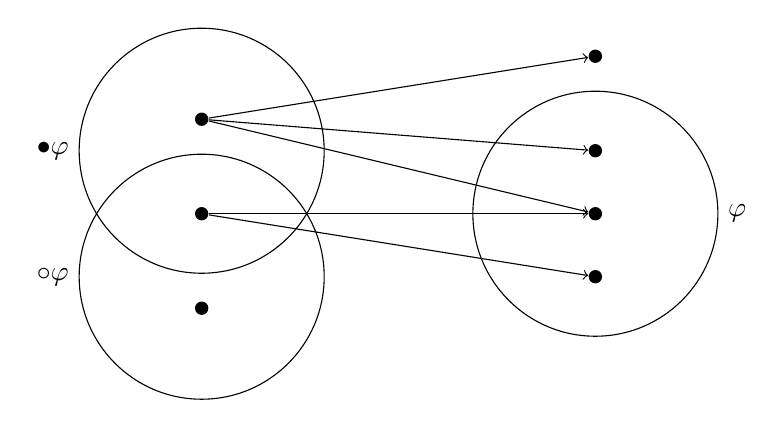
\begin{tikzpicture}
	\node at (2,1.2)[circle,draw,inner sep=1.1cm,label=left:$\wnext \varphi$] 
	{};
	\node at (2,2.8)[circle,draw,inner sep=1.1cm,label=left:$\snext \varphi$] 
	{};
	\node at (7,2)  [circle,draw,inner sep=1.1cm,label=right:$\varphi$] {};
	\node (down) at (2,0.8) [circle,fill=black,inner sep=0.6mm] {};
	\node (middle) at (2,2) [circle,fill=black,inner sep=0.6mm] {};
	\node (up) at (2,3.2) [circle,fill=black,inner sep=0.6mm] {};
	\node (r0) at (7,4) [circle,fill=black,inner sep=0.6mm] {};
	\node (r1) at (7,2.8) [circle,fill=black,inner sep=0.6mm] {};
	\node (r2) at (7,2) [circle,fill=black,inner sep=0.6mm] {};
	\node (r3) at (7,1.2) [circle,fill=black,inner sep=0.6mm] {};
	\draw [->] (middle) to (r2);
	\draw [->] (middle) to (r3);
	\draw [->] (up) to (r0);
	\draw [->] (up) to (r1);
	\draw [->] (up) to (r2);
	\end{tikzpicture}
	\caption{Strong next $\snext \varphi$ and weak next $\wnext \varphi$.}
	\label{fig:snext-vs-wnext}
\end{figure}

\subsection{Language semantics as transition system}
A Language semantics can be seen as the definition of a transition system.
In \K framework (\url{http://kframework.org}), a language semantics is defined as a finite set of \emph{reachability rules} over the signature $\sig^\RS = \sig^\cfg \cup \{ \snext \in \Sigma_{ \Cfg , \Cfg } \} $.
$\sig^\cfg$ is the signature of \emph{static program configurations}. 
It may have various sorts and symbols, among which there is a distinguished sort~$\Cfg$.
Fix a $\sig^\cfg$-model $M^\cfg$ and $M^\cfg_\Cfg$ is the set of all configurations.
\emph{Reachability rules}, or simply \emph{rules} have the form
$\varphi_1 \To \varphi_2$, where $\varphi_1,\varphi_2$ are $\sig^\cfg$-patterns (without $\mu$).
A reachability system yields a transition system $\Sbb = (M^\cfg_\Cfg,R)$ where
$s \mathbin{R} t$ if there exist a rule $\varphi_1 \To \varphi_2 \in S$
and an $M^\cfg$-valuation $\rho$ such that
$s \in \rhobar(\varphi_1)$ and $t \in \rhobar(\varphi_2)$.

In \mmul, we axiomatize the same transition system by:
\vspace*{-1ex}
\begin{itemize}
\item desugar each reachablitiy rule $\varphi_{l_i} \To \varphi_{r_i}$ to 
	  $\forall x_i \ldot \varphi_{l_i} \imp \snext \varphi_{r_i}$, $x_i \in \FV(\varphi_{l_i})$
\item introduce a \emph{STEP} axiom schema synthesized from all the rules in the semantics: 
\begin{align*}
\varphi \imp \wnext \bigvee_{i=1} \exists x_i \ldot \ceil{\varphi_{l_i} \wedge \varphi} \wedge \varphi_{r_i}
\end{align*}
$\varphi$ is an arbitrary pattern of sort $\Cfg$.
\end{itemize}
We denote the resulting $\sig^\TS$-theory $\Gamma^\Lang$.
The set of ``one-step'' axioms describes what should be included in the transition relation $R$.
The \emph{STEP} axiom ensures that no junk is added to the transition relation $R$.
It is equivalent to say that the transition relation $R$ is the \emph{least} set that satisfies the reachability rules.
Note that given the current configuration $\varphi$, $\varphi_w = \bigvee_{i=1} \exists x_i \ldot \ceil{\varphi_{l_i} \wedge \varphi} \wedge \varphi_{r_i}$ captures the \emph{least} set among all $\varphi'$ such that $\varphi \imp \wnext \varphi'$ holds.

\subsection{Defining \ModmuL in \MmuL} \label{subsec: defining_modmul}

Modal $\mu$-logic can be regarded as an empty theory in a vanilla \mmul without quantifiers, over a signature containing only one sort and only one symbol, which is unary.
When reasoning about programs and their properties, we need to extend proposition variables in $\PVar$ to arbitrary static program configuration pattern of sort \emph{$\Cfg$}.
Since we regard propositional variables in $\PVar$ as \mmul set variables when defining the transition systems, it is safe to do so with any modification.
We can add more temporal modalities as derived constructs:

\vspace*{-3ex}
\begin{align*}
\text{``eventually''} &\ 
\eventually \varphi \equiv \mu X \ldot\, \varphi \vee \snext X
\\
\text{``always''} &\ 
\always \varphi \equiv \nu X \ldot\, \varphi \wedge \wnext X
%\end{align*}
%\begin{align*}
\\
\text{``(strong) until''}  &\ 
\varphi_1 \until \varphi_2 \equiv 
\mu X \ldot\, \varphi_2 \vee (\varphi_1 \wedge \snext X)
\\
\text{``well-founded''} &\
\wellfounded \equiv \mu X \ldot \wnext X
\quad\text{\doubleslash no infinite paths}
\end{align*}
\vspace*{-5ex}

\noindent
Note that these definitions work on general transition systems and there is no requirement on the model to be \emph{linear future} or \emph{infinite future} (e.g., \LTL).
We can use the same pattern to reason about transition systems that have terminating states.

\subsection{\BMC as Proof-Searching in $\PS_\mu$}

The above sections suggests that \mmul may offer a unifying playground to
specify and reason about transition systems, by means of $\sig^\TS$-theories/models.
As a result, we can specify the program configurations and their properties as \mmul pattern and reason about the validity of the pattern in the proof system $\PS_\mu$.

Since dealing with \modmul in general is hard, we only consider some special cases.
We assume that the pattern is of the form $\varphi_\init \imp \varphi_\prop$.
$\varphi_\init$ is a static configuration pattern(i.e., without $\mu$ or \emph{next} symbol), which represents a set of initial configuration.
Especially, we require the $\varphi_\init$ to be of the form $\varphi_1 \vee \cdots \vee \varphi_n$, where $\varphi_i = t_i(x) \wedge p_i(x)$.
$t_i(x)$ is a pattern formed only with configuration constructors, domain values and variables. 
$p_i(x)$ is a predicate over variables.
$\varphi_\prop$ encodes the temporal property that we want to check.
It is a pattern of the form $\mu X \ldot \, \varphi_\sub$ (or $\nu X \ldot \, \varphi_\sub$). 
Moreover, we have four additional requirements on $\varphi_\sub$:
\begin{itemize}
\item $\varphi_\sub$ does not contain $\mu$, $\nu$ or $\snext$, but $\wnext$ is allowed.
\item set variable $X$ only appears under $\wnext$.
\item $\neg$ only appears before static configuration sub-patterns~\footnote{patterns do not contain $\mu$, $\nu$ or $\snext$-derived symbols}.
\item sub-patterns of $\varphi_\sub$ do not have form $\wnext \varphi_1 \vee \wnext \varphi_2$
\end{itemize}
Also, we require that $X$ only appears under $\wnext$ in $\varphi_\sub$ and $\neg$ does not appear before $\wnext$ or $X$.
For example, given the $\IMP$ semantics~\footnote{\url{https://github.com/kframework/k/blob/master/k-distribution/tutorial/1_k/2_imp/lesson_5/imp.k}}, the following pattern checks the \emph{non-division-by-zero} property~\footnote{$\always$ is a derived construct defined in Section~\ref{subsec: defining_modmul}}:
\begin{lstlisting}
    (<k> while (true) { 
           n = 100 / i;
           i = i + -1; } ~> K1 </k>
     <state> n |-> N:Int i |-> I:Int </state> $\wedge$ I > 5)
$\imp \always$ ($\forall{X} \ldot \forall{Y} \ldot \forall{K2} \ldot \forall{S} \ldot$
        (<k> X:Int / Y:Int ~> K2 </k> 
         <state> S </state>) $\imp$ Y =/= 0)
\end{lstlisting}

Given the search depth \emph{k}, bounded model checking the pattern $\varphi_\init \imp \varphi_\prop$ can be seen as a fully automatic procedure to derive the proof tree of the pattern in the proof system $\PS_\mu$ by limiting the depth of the proof tree.
Since we only consider the finite future (bounded by depth \emph{k}) of the model,
we can simply use $\nabla X \ldot \varphi = \varphi [ \nabla X \ldot \, \varphi / X ]$, where $\nabla \in \{ \mu, \nu \}$, to unroll the fixpoint pattern without worrying about whether it is a least or a greatest fixpoint.

\begin{algorithm}
\SetKwData{cGoals}{cGoals}
\SetKwData{nGoals}{nGoals}
\SetKwData{dep}{depth}
\SetKwData{Proved}{Proved}
\SetKwData{Failed}{Failed}
\SetKwData{Unknown}{Unknown}
\KwIn{$\varphi_\init \imp \varphi_\prop$, Axiom set $\Gamma^\Lang$, Depth D}
\KwOut{\Proved, \Failed Or \Unknown}

$\cGoals = \{\varphi_\init \imp \varphi_\prop\}$\;
$\nGoals = \emptyset$\;
$\dep = 0$\;
\While{$\dep \leq D$}{
	increment $\dep$\;
	\If{\cGoals is $\emptyset$}{
		return \Proved\;
	}
	\While{$\cGoals \neq \emptyset$}{
	    pick $\; \varphi_l \imp \varphi_r \;$ from $\cGoals$, $\cGoals = \cGoals \setminus \{ \varphi_l \imp \varphi_r \}$\;
	    \uIf{$\varphi_l = \varphi_{l_1} \vee \cdots \varphi_{l_n}$}{
	    	\tcp{case analysis}
	    	$\cGoals = \cGoals \cup \{ \varphi_{l_1} \imp \varphi_r, \cdots, \varphi_{l_n} \imp \varphi_r \}$\;
	    }
        \uElseIf{$\varphi_r$ doesn't contain $\wnext$ operator}{
        	encode $\neg(\varphi_l \imp \varphi_r)$ in Z3\;
        	\If{sat}{
        		return \Failed\;
            }
        }
    	\uElseIf{$\varphi_r = \varphi_{r_1} \wedge \varphi_{r_2}$}{
    		$\cGoals = \cGoals \cup \{ \varphi_l \imp \varphi_{r_1}, \cdots, \varphi_n \imp \varphi_{r_2} \}$\;
    	}
        \uElseIf{$\varphi_r = \varphi_{r_1} \vee \varphi_{r_2}$ and $\varphi_{r_1}$ doesn't contain $\wnext$ operator}{
        	$\cGoals = \cGoals \cup \{ (\varphi_l \wedge \neg \varphi_{r_1}) \imp \varphi_{r_2} \}$\;
        }
        \uElseIf{$\varphi_r = \nabla X \ldot \varphi$}{
        	$\cGoals = \cGoals \cup \{ \varphi_l \imp \varphi [ \nabla X \ldot \, \varphi / X ] \}$\;
        }
        \uElseIf{$\varphi_r = \wnext \varphi$}{
        	compute $\varphi_w$ using \emph{STEP} axiom in $\Gamma^\Lang$\;
        	$\nGoals = \nGoals \cup \{ \varphi_w \imp \varphi \}$
        }
   }
   $\cGoals = \nGoals$\;
   $\nGoals = \emptyset$\;
}
\eIf{\cGoals is $\emptyset$}{
	return \Proved\;
}{ return \Unknown\; }
\caption{Bounded Model Checking} \label{algorithm:BMC}
\end{algorithm}

The bounded model checking algorithm is described in the Algorithm~\ref{algorithm:BMC}.
The algorithm uses the proof rules in $\PS_\mu$ to derive the sub proof goals of the form $\varphi_{l'} \imp \varphi_{r'}$from the current proof goal.
Conceptually, it keeps doing equivalent rewriting of the current proof goal and separate sub proof goals $\varphi_{l'} \imp \varphi_{r'}$ into:

\vspace{-1ex}
\begin{enumerate}[label=(\roman*), leftmargin=2\parindent]
\item $\varphi_{r'}$ does not contain $\wnext$ operator.
      We can check its validity in the current iteration.
\item $\varphi_{r'}$ does contain $\wnext$ operator.
      We can only check its validity in the future iteration.
\end{enumerate}
\vspace{-1ex}

\noindent
For condition (\rmnum{1}), we can directly encode the pattern as Z3 query and check its validity.
For condition (\rmnum{2}), we use \emph{STEP} axiom to compute the ``precise'' pattern $\varphi_{w'}$ that represents the ``all-path next'' states of $\varphi_{l'}$.
Since $\varphi_{l'} \imp \wnext \varphi_{w'}$, we only need to prove $\wnext \varphi_{w'} \imp \wnext \varphi$ in order to prove $\varphi_{l'} \imp \wnext \varphi$. By applying \framing rule, we only need to prove $ \varphi_{w'} \imp \varphi$ in the next iteration.
Note that the depth D in the bounded model checking algorithm constraints the maximum number of $\wnext$ computed in each path starting from the root in the proof tree.

\begin{figure}[!ht]

\begin{displaymath}
\prftree
{\prftree
 {\prftree
  {\cdots}
  {\varphi_l \imp \varphi}
 }
 {\prftree[r]{\modusponens}
  {\prftree[r]{\step}
   {\cdot}
   {\varphi \imp \wnext \varphi_w}
  }
  {\prftree[r]{\framing}
   {\prftree
   	{\cdots}
   	{\varphi_w \imp \mu X \ldot \varphi \wedge \wnext X}
   }
   {\wnext \varphi_w \imp  \wnext (\mu X \ldot \varphi \wedge \wnext X)}
  }
  {\varphi_l \imp \wnext (\mu X \ldot \varphi \wedge \wnext X)}
 }
 {\varphi_l \imp \varphi \wedge \wnext (\mu X \ldot \varphi \wedge \wnext X)}
}
{\varphi_l \imp \mu X \ldot \varphi \wedge \wnext X}
\end{displaymath}
\caption{sub proof tree of the pattern $\varphi_l \imp \mu X \ldot \varphi \wedge \wnext X$}
\label{fig:proof-tree}
\end{figure}

As an example, Figure~\ref{fig:proof-tree} shows part of the proof tree for the pattern $\varphi_l \imp \mu X \ldot \varphi \wedge \wnext X$.
If $\varphi_l$ does not have successors, $\varphi_w$ becomes $\bot$ and $\varphi_w \imp \mu X \ldot \varphi \wedge \wnext X$ becomes $\top$ immediately.

\subsection{Prototype and Result}
I prototyped the above algorithm in the \K haskell-backend~\footnote{\url{https://github.com/kframework/kore}}.
In the prototype, I focused on the pattern $\varphi_\init \imp \always (\forall X \ldot \varphi_\pattern(X) \imp \varphi_\predicate(X))$.
It is a very general global invariant pattern which can be used to check that $\varphi_\predicate(X)$ holds on every reachable state that matches $\varphi_\pattern(X)$ from the initial state $\varphi_\init$.
Properties such as \emph{non-division-by-zero} and \emph{assertions} can be encoded in this pattern.

My prototype can work on some simple semantics like $\IMP$ in the \K framework.
In one example, the prototype takes 311 seconds to explore 4494 symbolic states and sends over 14000 queries to Z3 solver~\cite{DBLP:conf/tacas/MouraB08}.
The initial results show that there is large room for improving the performance of the bounded model checker.

\section{Proposed Work}

Before highlighting the plans for the rest of the thesis work, below is a summary of part of the thesis work accomplished so far:

\begin{itemize}
\item I worked on improving the performance of runtime verification technique and applying runtime verification to the robot domain.
\item I helped to apply the \K' deductive program verifiers to high-profile commercial smart contracts and demonstrate its scalability and practicality.
\item I defined programming language semantics as transition systems in the \mmul.
I formalized the bounded model checking as a proof searching problem in the \mmul.
I proposed an algorithm to do bounded model checking on many general patterns.
\item I implemented a bounded model checker for all languages in the \K haskell backend.
I evaluated the checker on some simple semantics such as IMP.
\end{itemize}

The remaining part of the thesis work is about making the bounded model checker scalable and practical.

\begin{itemize}
\item To improve the performance of the bounded model checker.
In the initial experiment, I found that most of the time is spent on querying Z3~\cite{DBLP:conf/tacas/MouraB08}.
I plan to do most of the reasoning locally and minimize the queries that are sent to Z3.
What's more, I can take advantage of Z3's incremental solving ability to compute the ``weak next'' pattern faster by pushing and popping the conditions of the semantics rules.
\item To evaluate the bounded model checker on real-world semantics such as KEVM~\cite{KEVM}.
The KEVM semantics is actively developed and used to verify several high-profile smart contracts.
The ability to work with KEVM can demonstrate the scalability and practicality of the checker.
\item To \emph{conceptually} compare our approach with some existing bounded model checker such as CBMC~\cite{Clarke2004ATF} and CORRAL~\cite{corral-a-solver-for-reachability-modulo-theories-2}.
\item To generate the proof object after model checking a pattern.
If the bounded model checker returns \emph{Failed}, it should provide a concrete counter-example to the user.
If the checker returns \emph{Proved} or \emph{Unknown}, it should output the whole proof tree as the proof object.
\item To model various abstraction and reduction techniques in the literature as proof strategy or theory transformations to the original semantics.
On one hand, when deriving the sub-proof goals, instead of using the $\varphi_w$ pattern for computing the exact weak next states, we can use patterns in the abstract domain.
This maintains over-approximations for the reachable states.
On the other hand, we can do theory transformation on the original operational semantics to reduce the size of the transition system while preserving the property to check.
~\cite{MaudePOR} demonstrates a similar approach in the context of partial order reduction~\cite{Alur:2001:PRS:375503.375505,Flanagan:2005:DPR:1040305.1040315} for rewriting semantics of programming languages.

\end{itemize}


\section{Related Work}

I present related work for runtime verification, program verification and bounded model checking.

\subsection{Runtime Verification}
Runtime Verification (RV)~\cite{RuleBasedMOP,BoddenMOPBOxRV11,BoddenEtAlTraceMatches07,ChenAndRosuTowardsMOP03,DwyerETALOptimizing2010,HavelundRosuRV2001JPAX,HavelundRosuASE2001MonitoringProgramsUsingRewriting,JinEtAlJavaMOPToolPaperICSE12} is a technique for monitoring program executions against formal properties.
The general idea is that the RV tool instruments the program based on the properties so that executing instrumented programs generates appropriate events and creates \emph{monitors} to listen to events and check the properties.
Since the first papers on RV~\cite{HavelundRosuASE2001MonitoringProgramsUsingRewriting,HavelundRosuRV2001JPAX}, many techniques and tools were proposed in almost two decades.
One direction of the research in RV focuses on reducing the time and memory overhead during execution~\cite{JinEtAlGarbageCollectionPLDI2011,PurandareEtAlCompactionISSTA2013,DeckerETALTACAS2016MonitoringWithUnionFind,LuoETAlRVMonitor14,PurandareEtAlStutterEquivalentLoops2010} and supporting different formalism~\cite{MeredithRosuMonitoringStringRewritingASE13,MeredithETALMOPContextFreePatterns08,BarringerETALJLC2010EagleToRuler,HavelundETALFMCAD2017MonitoringWithBDDs}.
Another direction of research aims to apply RV techniques to various domains such as testing~\cite{LegunsenEtAleMOP15} and robot~\cite{huang-erdogan-zhang-moore-luo-sundaresan-rosu-2014-rvtool}.
However, little attention is paid to the correctness of the monitors themselves.
Our bounded model checking approach can also be used in runtime verification.
All we need to do is to encode the program and the concrete input in $\varphi_\init$ and set the search depth to infinity.
Our approach will work no matter $\varphi_\init$ is concrete or symbolic.
The advantage of our approach is that there is no need to trust the monitor code and the instrumentation tools, as a proof object will be generated during the execution.

Most of the RV tools translate the properties into state machines and generate monitor codes based on the state machines.
For properties written in extended regular expressions and linear temporal logic, \cite{sen-rosu-2003-rv,sen-rosu-agha-2003-asian} proposed a novel approach which uses \emph{derivatives} to generate automata as monitors.
In our approach, unrolling the $\mu$ binder is similar to calculating the derivatives.
However, we unroll the program and the property on the fly during the execution instead of constructing the automata in advance.

\subsection{Program Verification}
Program Verification uses formal methods of mathematics to prove the correctness of a program.
A popular approach to building program verifiers for real-world language is to translate to an intermediate verification language (IVL) and do verification at the IVL level.
This advantage of this approach is that VC generation and reasoning about state properties are implemented only once, at the IVL level.
Boogie~\cite{boogie} is a popular IVL integrated with Z3.
There are several verifiers built on top of Boogie, such as VCC~\cite{DBLP:conf/tphol/CohenDHLMSST09}, HAVOC~\cite{Havoc}, and
Dafny~\cite{DBLP:conf/lpar/Leino10}.
VCDrayd~\cite{DBLP:conf/pldi/PekQM14} is a separation logic based verifier built on top of VCC.
Another approach advocates to develop language-independent formal methods ~\cite{rosu-stefanescu-2012-icalp,rosu-stefanescu-2012-fm,rosu-stefanescu-2012-oopsla,rosu-stefanescu-ciobaca-moore-2013-lics,stefanescu-ciobaca-mereuta-moore-serbanuta-rosu-2014-rta} and reason about programs directly over \emph{operational semantics}.
This approach reduces the burden to specify multiple semantics and prove their soundness with respect to the operational semantics.

Our model checking technique follows the philosophy of the second approach and blurs the boundary between model checking and theorem proving.
In fact, all path reachability formula $\varphi \Rightarrow^\forall \varphi'$ can be expressed in the \mmul as $\varphi \imp \nu X \ldot \varphi' \vee (\wnext X \wedge \snext \top)$.
In other words, our bounded model checking can be seen as a fully \emph{automatic} proof tactics for proving patterns in \mmul.

\subsection{Model Checking}

Model checking~\cite{Clarke:2000:MC:332656} has been used extensively to algorithmically check temporal properties of models.
The literature on model checking is rich.
We only discuss work on symbolic software model checking.

There are several model checkers for different languages.
CBMC~\cite{Clarke2004ATF}, ESBMC~\cite{ESBMC},  Saturn~\cite{DBLP:conf/popl/XieA05} are widely used BMC tools for C programs.
CBMC has both SAT-based and SMT-based backend.
ESBMC is an SMT-based model checker which provide more accurate support for bit-level, pointers, unions and fixed point arithmetic.
Saturn improves upon the basic bounded model checking algorithm by computing and memoizing relations between inputs and outputs (“summaries”) for procedures bottom-up in the call graph.
This makes bounded model checking scale to large programs.
JavaPathFinder~\cite{Havelund2000} is an execution-based model checker for muilti-threaded Java programs that combines exploring schedule choices explicitly with tracking user inputs symbolically.
CORRAL~\cite{corral-a-solver-for-reachability-modulo-theories-2} is a bounded model checker for Boogie~\cite{boogie} programs where the depth of recursion is bounded by a user-supplied recursion bound.
It combines summaries, variable abstraction, and stratified inlining to solve the
reachability-modulo-theories problem.
The tools mentioned above were developed for a fixed target language and the language semantics is usually hardcoded within the implementation of their algorithms.
On the contrary, our approach works for all languages and is faithful to the operational semantics of the target language.

For infinite state programs, symbolic model checking may not terminate, or take
an inordinate amount of time or memory to terminate.
Various abstraction technique were proposed to trade off precision of the analysis for efficiency.
In practice, a well known approach is counterexample-guided abstraction refinement (CEGAR)~\cite{CEGR}.
The SLAM model checker~\cite{SLAM} was the first implementation of CEGAR with predicate abstraction for C programs.
Following SLAM project, BLAST~\cite{Henzinger:2002:LA:503272.503279} implements an optimization of CEGAR called lazy abstraction where the refinement step triggers the re-abstraction of only relevant parts of the original program.
CEGAR has been generalized to check properties of heap-manipulating programs~\cite{10.1007/978-3-642-12029-9_19}, as well as concurrent programs~\cite{Chaki:2003:MVS:776816.776863}.
It is interesting to see how these techniques can be incorporated as proof search strategy in our model checker.

\section{Conclusion}
The goal of my thesis is to demonstrate and improve the scalability and
practicality of the language-independent bounded model checker.
To support this, I worked on the underlying theories and came up with an algorithm to bounded model check specific forms of \modmul patterns.
I implemented the idea in the \K haskell-backend and made it work on simple language semantics such as IMP.
I will thoroughly evaluate the model checker on real world language and applications.
I believe that this approach reduces the trust base of the tool and would eliminate the need for dedicated model checkers for different languages.


\bibliographystyle{plain}
\bibliography{ref}

\end{document}
